\documentclass{article}
\usepackage{amsmath}
\usepackage{bm}
\usepackage{graphicx} 
\usepackage{lipsum}
\usepackage{caption} % Add this package

\begin{document}
	
	\section{Homogeneous Notation}
	
	\begin{center} 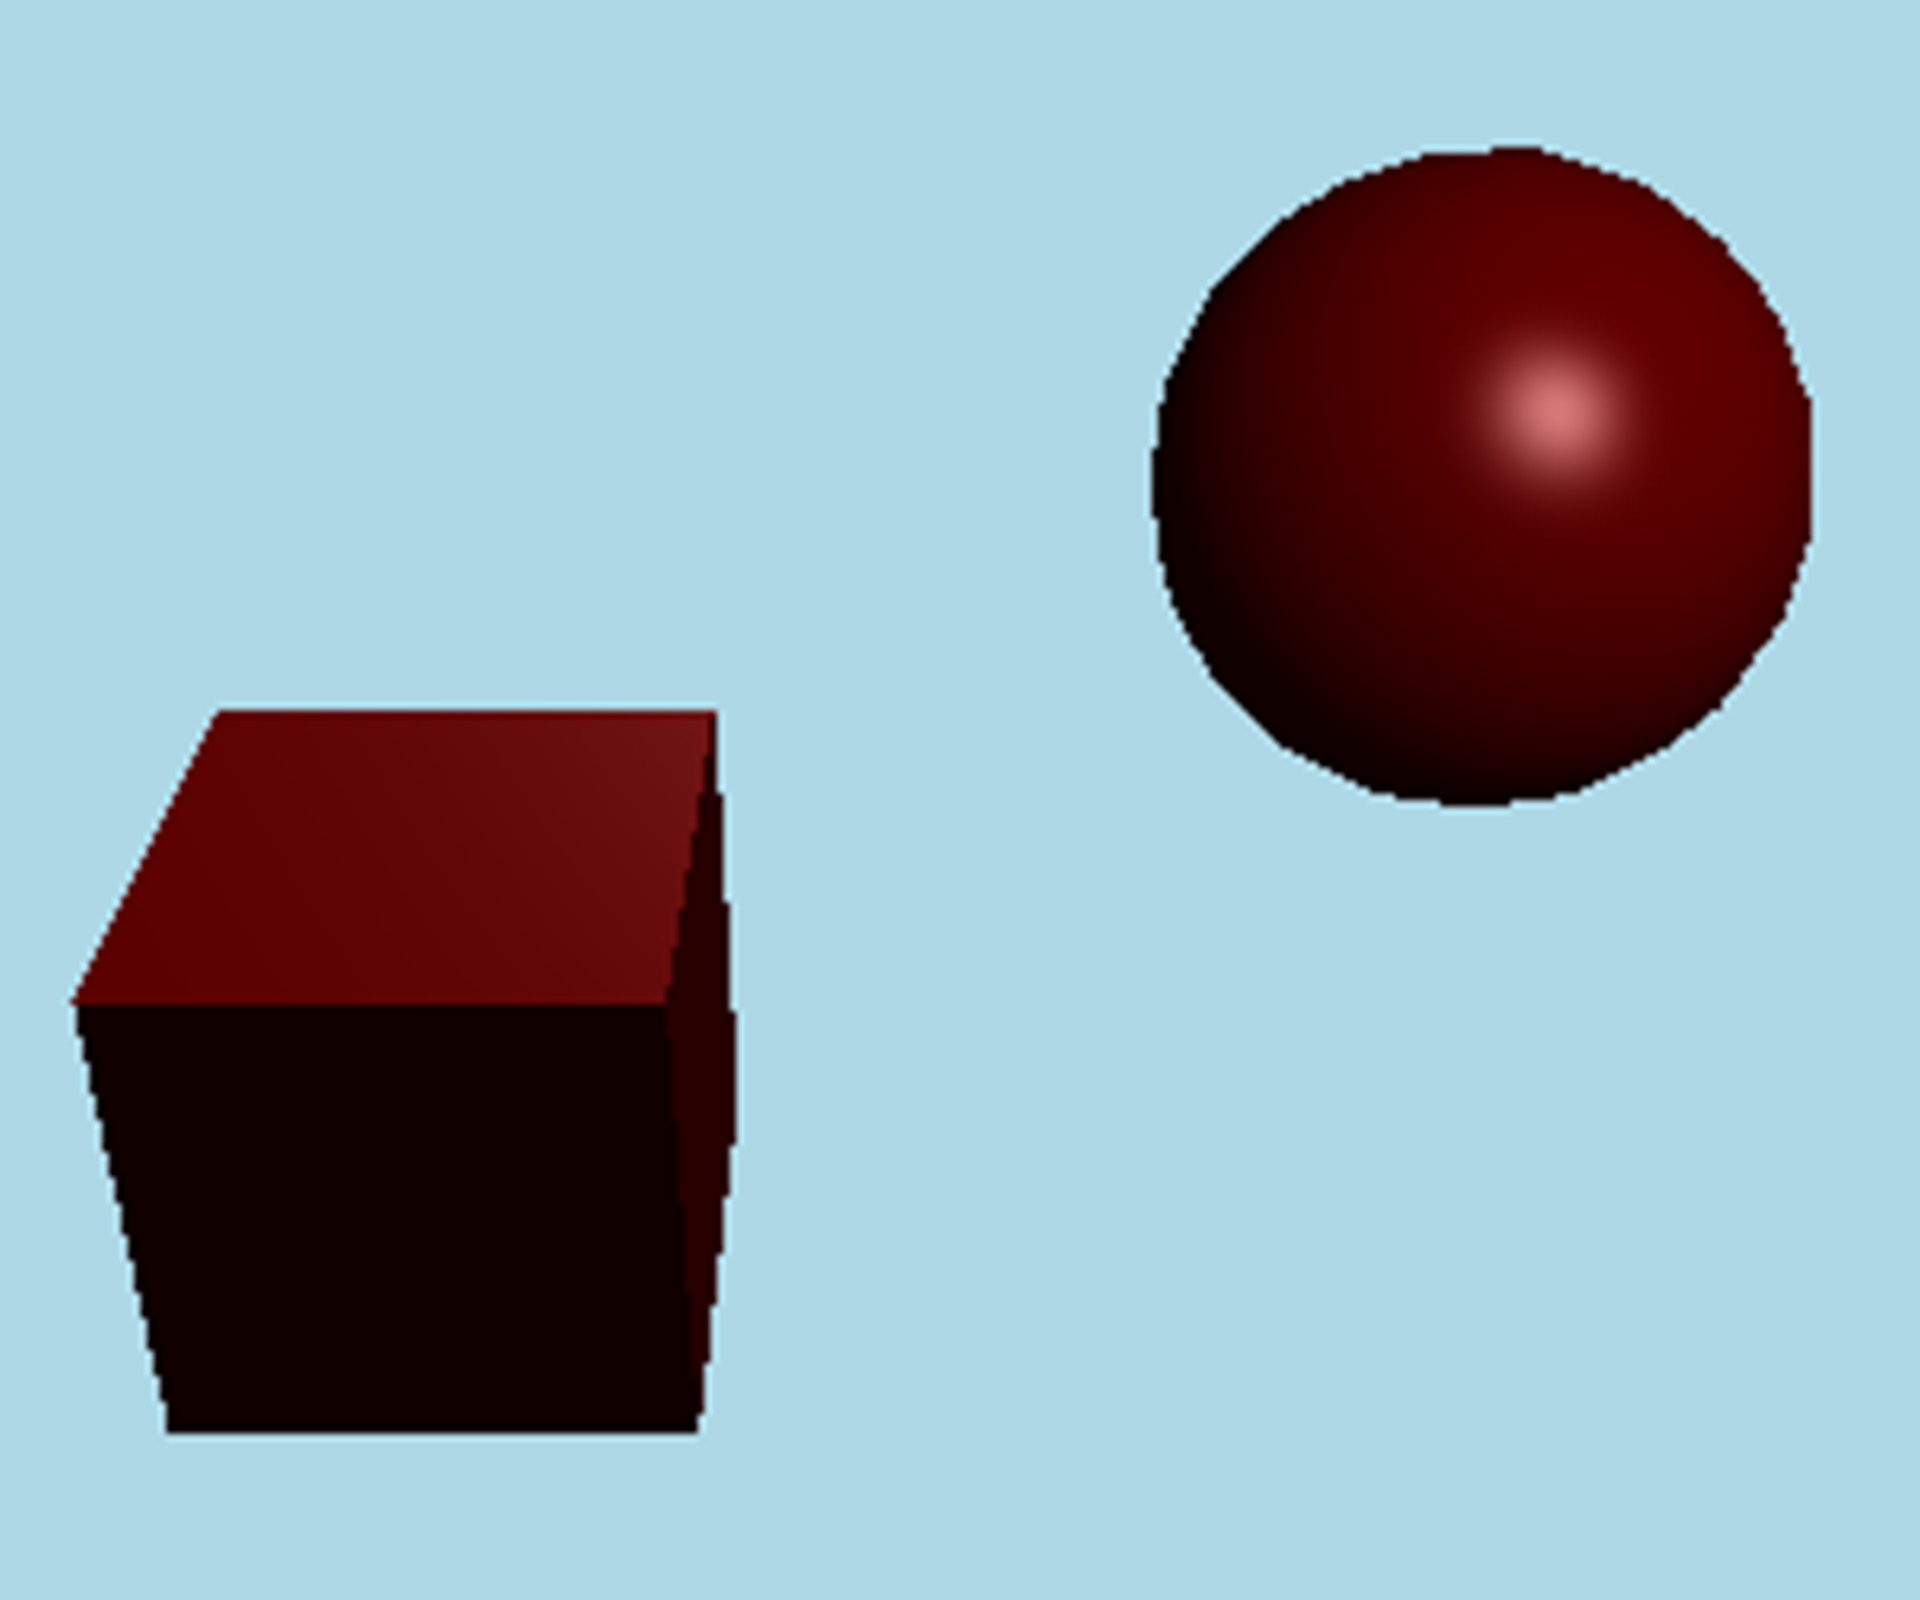
\includegraphics[width=1\textwidth]{homogenious_notation_images/transformation_all.jpg} \captionof{figure}{Different transformations are applied to cube and sphere} \end{center}
	
	\subsection{Homogeneous Notation for a Point}
	In homogeneous coordinates, a point \(\bm{p}\) in 3D space is represented as a 4D vector: \(\bm{p} = \begin{bmatrix} x \\ y \\ z \\ w \end{bmatrix}\).
	
	\subsection{Translation}
	To translate a point by a vector \(\bm{t} = \begin{bmatrix} t_x & t_y & t_z \end{bmatrix}^T\), I use the translation matrix \(\bm{T}\):
	
	
	\[
	\bm{T} = \begin{bmatrix}
		1 & 0 & 0 & t_x \\
		0 & 1 & 0 & t_y \\
		0 & 0 & 1 & t_z \\
		0 & 0 & 0 & 1
	\end{bmatrix}
	\]
	
	
	The translated point \(\bm{p}'\) is obtained by: \(\bm{p}' = \bm{T} \bm{p}\).
	

	\begin{center} 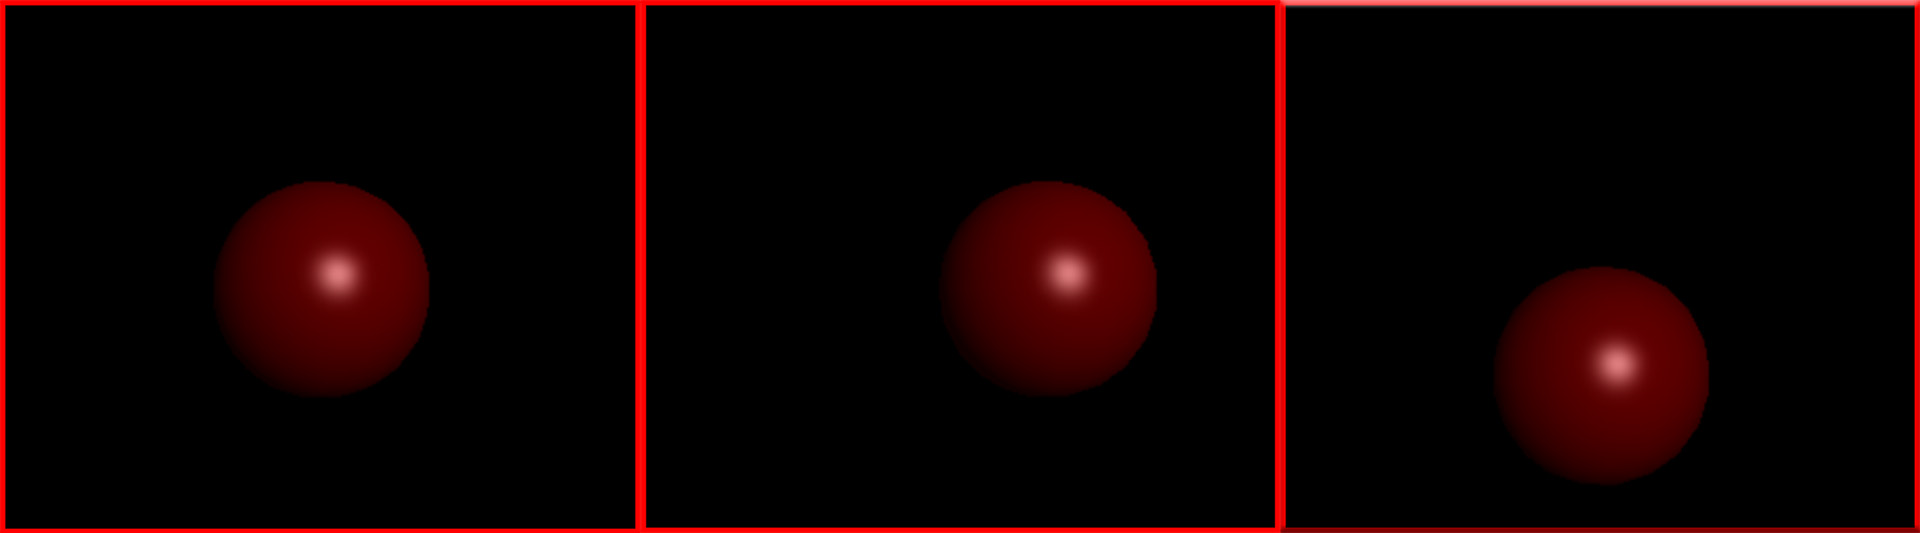
\includegraphics[width=1\textwidth]{homogenious_notation_images/position.jpg} \captionof{figure}{The sphere's position changes: in the middle, it moves to the right; on the left, it moves down.} \end{center}
	
	\subsection{Scaling}
	To scale a point by factors \(s_x\), \(s_y\), and \(s_z\), I use the scaling matrix \(\bm{S}\):
	
	
	\[
	\bm{S} = \begin{bmatrix}
		s_x & 0 & 0 & 0 \\
		0 & s_y & 0 & 0 \\
		0 & 0 & s_z & 0 \\
		0 & 0 & 0 & 1
	\end{bmatrix}
	\]
	
	
	The scaled point \(\bm{p}'\) is obtained by: \(\bm{p}' = \bm{S} \bm{p}\).
	
\begin{center} 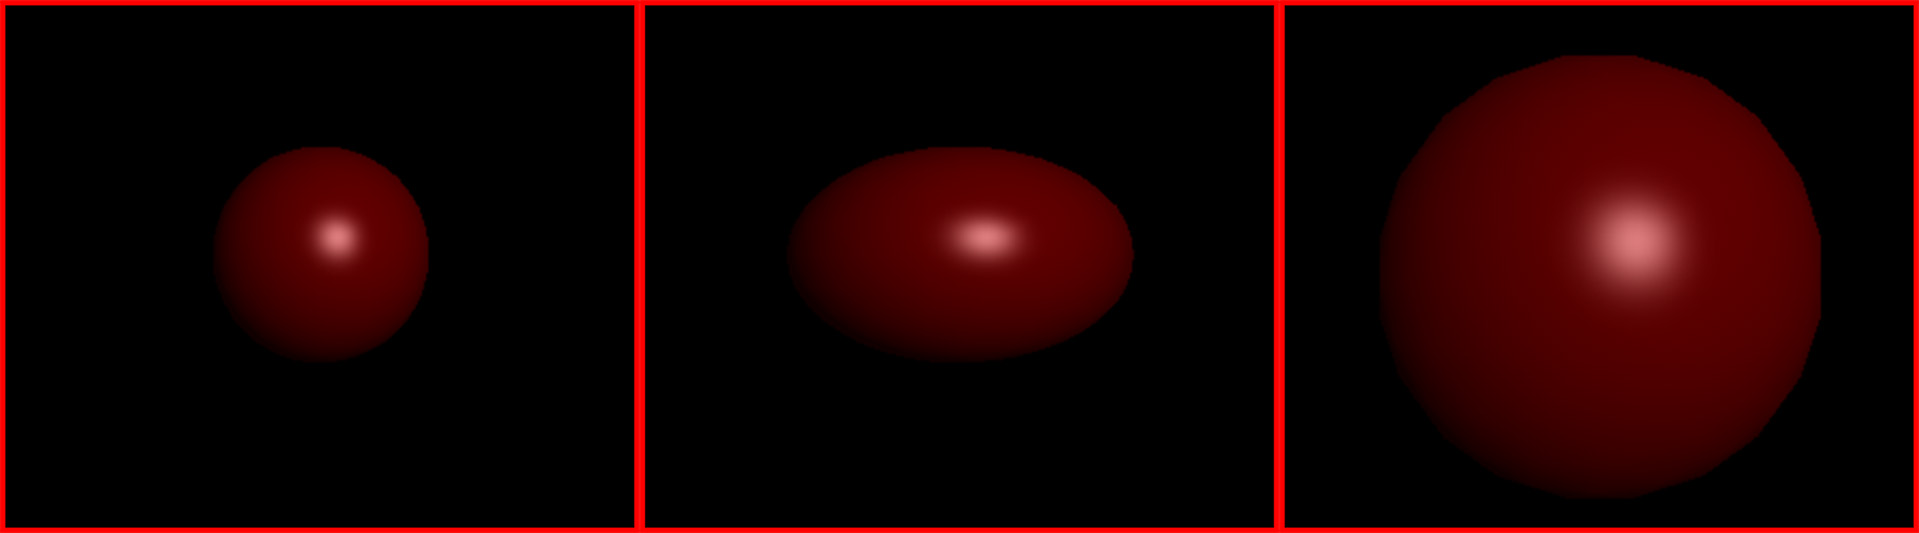
\includegraphics[width=1\textwidth]{homogenious_notation_images/scale.jpg} \captionof{figure}{Sphere is scaled in x direction and is scaled by 2.} \end{center}
	\subsection{Mirroring}
	To mirror a point along the \(x\), \(y\), or \(z\) axis, I use the mirroring matrices \(\bm{M}_x\), \(\bm{M}_y\), and \(\bm{M}_z\):
	
	
	\[
	\bm{M}_x = \begin{bmatrix}
		-1 & 0 & 0 & 0 \\
		0 & 1 & 0 & 0 \\
		0 & 0 & 1 & 0 \\
		0 & 0 & 0 & 1
	\end{bmatrix}
	\quad
	\bm{M}_y = \begin{bmatrix}
		1 & 0 & 0 & 0 \\
		0 & -1 & 0 & 0 \\
		0 & 0 & 1 & 0 \\
		0 & 0 & 0 & 1
	\end{bmatrix}
	\quad
	\bm{M}_z = \begin{bmatrix}
		1 & 0 & 0 & 0 \\
		0 & 1 & 0 & 0 \\
		0 & 0 & -1 & 0 \\
		0 & 0 & 0 & 1
	\end{bmatrix}
	\]
	
	
	The mirrored point \(\bm{p}'\) is obtained by: \(\bm{p}' = \bm{M}_x \bm{p}\) or \(\bm{p}' = \bm{M}_y \bm{p}\) or \(\bm{p}' = \bm{M}_z \bm{p}\).

	\subsection{Rotation}
	To rotate a point around the \(x\), \(y\), or \(z\) axis by an angle \(\theta\), I use the rotation matrices \(\bm{R}_x\), \(\bm{R}_y\), and \(\bm{R}_z\):
	
	
	\[
	\bm{R}_x = \begin{bmatrix}
		1 & 0 & 0 & 0 \\
		0 & \cos \theta & -\sin \theta & 0 \\
		0 & \sin \theta & \cos \theta & 0 \\
		0 & 0 & 0 & 1
	\end{bmatrix}
	\quad 
	\]
	\[
	\bm{R}_y = \begin{bmatrix}
		\cos \theta & 0 & \sin \theta & 0 \\
		0 & 1 & 0 & 0 \\
		-\sin \theta & 0 & \cos \theta & 0 \\
		0 & 0 & 0 & 1
	\end{bmatrix} \]
	\[
	\quad
	\bm{R}_z = \begin{bmatrix}
		\cos \theta & -\sin \theta & 0 & 0 \\
		\sin \theta & \cos \theta & 0 & 0 \\
		0 & 0 & 1 & 0 \\
		0 & 0 & 0 & 1
	\end{bmatrix}
	\]
	
	
	The rotated point \(\bm{p}'\) is obtained by: \(\bm{p}' = \bm{R}_x \bm{p}\) or \(\bm{p}' = \bm{R}_y \bm{p}\) or \(\bm{p}' = \bm{R}_z \bm{p}\).
	
	\begin{center} 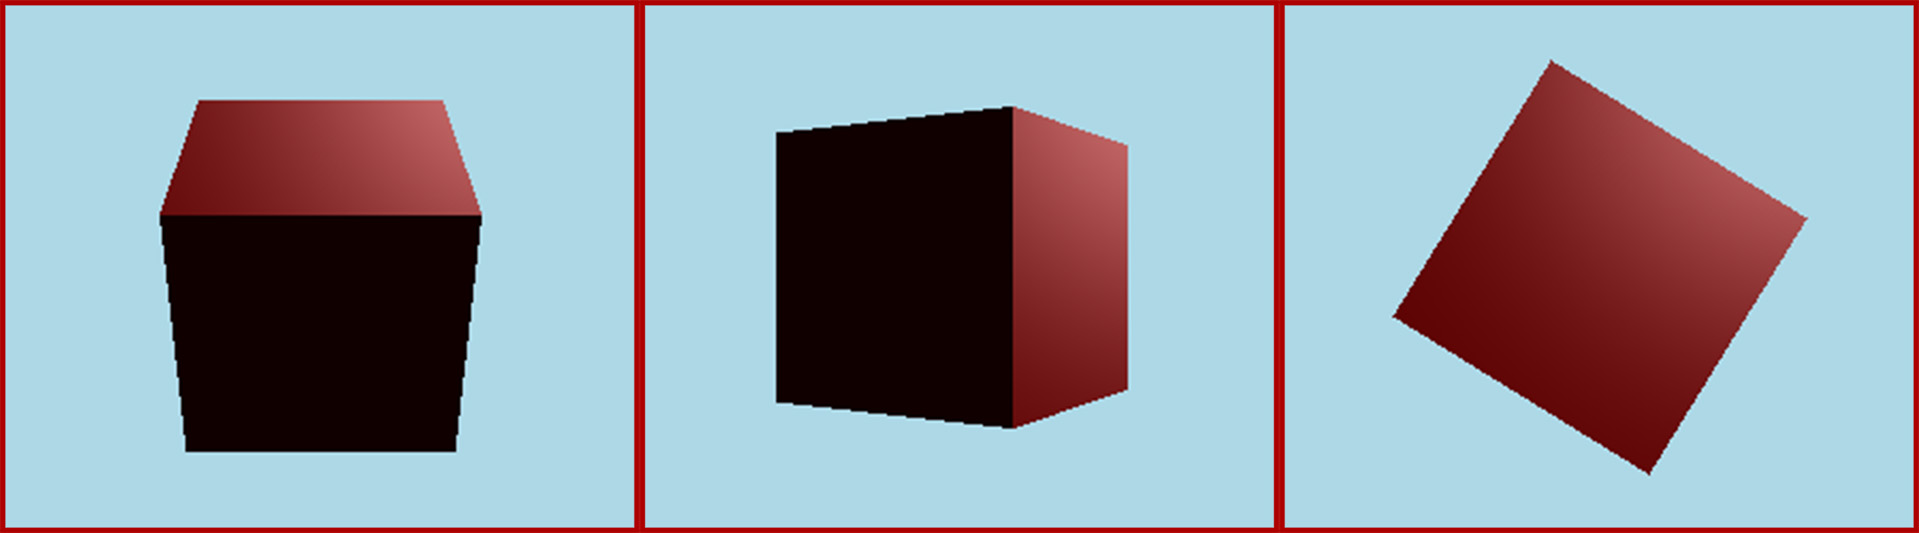
\includegraphics[width=1\textwidth]{homogenious_notation_images/rotate.jpg} \captionof{figure}{Cube is rotated by 45 Degrees in each direction.} \end{center}
		
	\subsection{Shearing}
	To shear a point along the \(x\), \(y\), or \(z\) axis, I use the shearing matrices \(\bm{H}_{xy}\), \(\bm{H}_{xz}\), \(\bm{H}_{yx}\), \(\bm{H}_{yz}\), \(\bm{H}_{zx}\), and \(\bm{H}_{zy}\):
	
	
	\[
	\bm{H}_{xy} = \begin{bmatrix}
		1 & h_{xy} & 0 & 0 \\
		0 & 1 & 0 & 0 \\
		0 & 0 & 1 & 0 \\
		0 & 0 & 0 & 1
	\end{bmatrix}
	\quad
	\bm{H}_{xz} = \begin{bmatrix}
		1 & 0 & h_{xz} & 0 \\
		0 & 1 & 0 & 0 \\
		0 & 0 & 1 & 0 \\
		0 & 0 & 0 & 1
	\end{bmatrix}
	\quad
	\bm{H}_{yx} = \begin{bmatrix}
		1 & 0 & 0 & 0 \\
		h_{yx} & 1 & 0 & 0 \\
		0 & 0 & 1 & 0 \\
		0 & 0 & 0 & 1
	\end{bmatrix}
	\]
	
	
	
	
	\[
	\bm{H}_{yz} = \begin{bmatrix}
		1 & 0 & 0 & 0 \\
		0 & 1 & h_{yz} & 0 \\
		0 & 0 & 1 & 0 \\
		0 & 0 & 0 & 1
	\end{bmatrix}
	\quad
	\bm{H}_{zx} = \begin{bmatrix}
		1 & 0 & 0 & 0 \\
		0 & 1 & 0 & 0 \\
		h_{zx} & 0 & 1 & 0 \\
		0 & 0 & 0 & 1
	\end{bmatrix}
	\quad
	\bm{H}_{zy} = \begin{bmatrix}
		1 & 0 & 0 & 0 \\
		0 & 1 & 0 & 0 \\
		0 & h_{zy} & 1 & 0 \\
		0 & 0 & 0 & 1
	\end{bmatrix}
	\]
	
	
	The sheared point \(\bm{p}'\) is obtained by: \(\bm{p}' = \bm{H}_{xy} \bm{p}\), \(\bm{p}' = \bm{H}_{xz} \bm{p}\), \(\bm{p}' = \bm{H}_{yx} \bm{p}\), \(\bm{p}' = \bm{H}_{yz} \bm{p}\), \(\bm{p}' = \bm{H}_{zx} \bm{p}\), or \(\bm{p}' = \bm{H}_{zy} \bm{p}\).
	
		\begin{center} 
\includegraphics[width=1\textwidth]{homogenious_notation_images/shear.jpg} \captionof{figure}{Cube is transformed with Shear} \end{center}
		
\end{document}
